\documentclass[portrait,a0paper]{baposter}

\usepackage[vlined]{algorithm2e}
\usepackage{times}
\usepackage{calc}
\usepackage{url}
\usepackage{graphicx}
\usepackage{amsmath}
\usepackage{amssymb}
\usepackage{relsize}
\usepackage{multirow}
\usepackage{booktabs}
\usepackage{multirow}
\usepackage{bbm}
\usepackage{bm}

\usepackage{graphicx}
\usepackage{multicol}
\usepackage[T1]{fontenc}
\usepackage{ae}
\usepackage{enumitem}

\usepackage{colortbl}
\usepackage{xcolor}
\graphicspath{{images/}}



\setlist[itemize]{leftmargin=*,nosep}
 \setlength{\columnsep}{0.7em}
 \setlength{\columnseprule}{0mm}

\usepackage[pdftex,
            pdfauthor={Zhipeng He},
            pdftitle={Investigating Imperceptibility of Adversarial Attacks on Tabular Data: An Empirical Analysis},
            pdfsubject={Research Poster for ADSN 2024},
            pdfkeywords={Adversarial Attacks, Tabular Data, Imperceptibility},
            pdfproducer={LaTex by Overleaf},
            pdfcreator={pdflatex}]{hyperref}
% %%%%%%%%%%%%%%%%%%%%%%%%%%%%%%%%%%%%%%%%%%%%%%%%%%%%%%%%%%%%%%%%%%%%%%%%%%%%%%%%
% % Save space in lists. Use this after the opening of the list
% %%%%%%%%%%%%%%%%%%%%%%%%%%%%%%%%%%%%%%%%%%%%%%%%%%%%%%%%%%%%%%%%%%%%%%%%%%%%%%%%
 \newcommand{\compresslist}{%
 \setlength{\itemsep}{0pt}%
 \setlength{\parskip}{0pt}%
 \setlength{\parsep}{0pt}%
 }
\renewcommand{\rmdefault}{ptm} % Arial
\renewcommand{\sfdefault}{ptm} % Arial

%%%%%%%%%%%%%%%%%%%%%%%%%%%%%%%%%%%%%%%%%%%%%%%%%%%%%%%%%%%%%%%%%%%%%%%%%%%%%
%% Begin of Document
%%%%%%%%%%%%%%%%%%%%%%%%%%%%%%%%%%%%%%%%%%%%%%%%%%%%%%%%%%%%%%%%%%%%%%%%%%%%%
\begin{document}
%%%%%%%%%%%%%%%%%%%%%%%%%%%%%%%%%%%%%%%%%%%%%%%%%%%%%%%%%%%%%%%%%%%%%%%%%%%%%
%% Here starts the poster
%%---------------------------------------------------------------------------
%% Format it to your taste with the options
%%%%%%%%%%%%%%%%%%%%%%%%%%%%%%%%%%%%%%%%%%%%%%%%%%%%%%%%%%%%%%%%%%%%%%%%%%%%%
\begin{poster}{
 % Show grid to help with alignment
 grid=false,
 columns=5,
 % Column spacing
 colspacing=0.7em,
 % Color style
 headerColorOne=cyan!20!white!90!black,
 borderColor=cyan!30!white!90!black,
 % Format of textbox
 textborder=faded,
 % Format of text header
 headerborder=open,
 headershape=roundedright,
 headershade=plain,
 background=none,
 bgColorOne=cyan!10!white,
 headerheight=0.09\textheight}
 % Eye Catcher
 {
      
\includegraphics[width=0.08\linewidth]{qut-logo-og-1200.jpg}
      % \makebox[0.01\textwidth]{} 
      \raisebox{-0.14\height}{
\includegraphics[width=0.11\linewidth]{uts_logo.jpg}}
      % \makebox[0.04\textwidth]{} 
 }
 % Title
 {
 {\sc\huge\bf Investigating Imperceptibility of Adversarial Attacks on Tabular Data: An Empirical Analysis}}
 % Authors
 {Zhipeng He$^1$, Chun Ouyang$^1$, Laith Alzubaidi$^1$, Alistair Barros$^1$, Catarina Moreira$^2$ \\[0.2em]
 {$^1$ Queensland University of Technology, $^2$ University of Technology Sydney}}
 % University logo
 {
    \begin{tabular}{r}
        
\includegraphics[width=0.08\linewidth]{ADSN-Logo-Black-Stacked.png}
    \end{tabular}
 }

%%%%%%%%%%%%%%%%%%%%%%%%%%%%%%%%%%%%%%%%%%%%%%%%%%%%%%%%%%%%%%%%%%%%%%%%%%%%%%
%%% Now define the boxes that make up the poster
%%%---------------------------------------------------------------------------
%%% Each box has a name and can be placed absolutely or relatively.
%%% The only inconvenience is that you can only specify a relative position 
%%% towards an already declared box. So if you have a box attached to the 
%%% bottom, one to the top and a third one which should be inbetween, you 
%%% have to specify the top and bottom boxes before you specify the middle 
%%% box.
%%%%%%%%%%%%%%%%%%%%%%%%%%%%%%%%%%%%%%%%%%%%%%%%%%%%%%%%%%%%%%%%%%%%%%%%%%%%%%

%%%%%%%%%%%%%%%%%%%%%%%%%%%%%%%%%%%%%%%%%%%%%%%%%%%%%%%%%%%%%%%%%%%%%%%%%%%%%%
\headerbox{\bf\color{blue} Problem Definition}{name=contribution,column=0,row=0,span=3}{
    \textbf{\color{blue}Background:} Adversarial attacks involve modifying input data to deceive machine learning models. These attacks have been studied for unstructured data (e.g., images), but structured tabular data poses unique challenges.

    \vspace{0.3em}
    \textbf{\color{blue}Gaps:} 1) The imperceptibility of adversarial attacks on tabular data requires approaching different concepts compared to those for images. 2) Current adversarial attacks lack imperceptibility metrics tailored for tabular data.
    
    \begin{center}
        \vspace{-2em}
    \begin{minipage}[b]{0.49\textwidth}
    \centering
    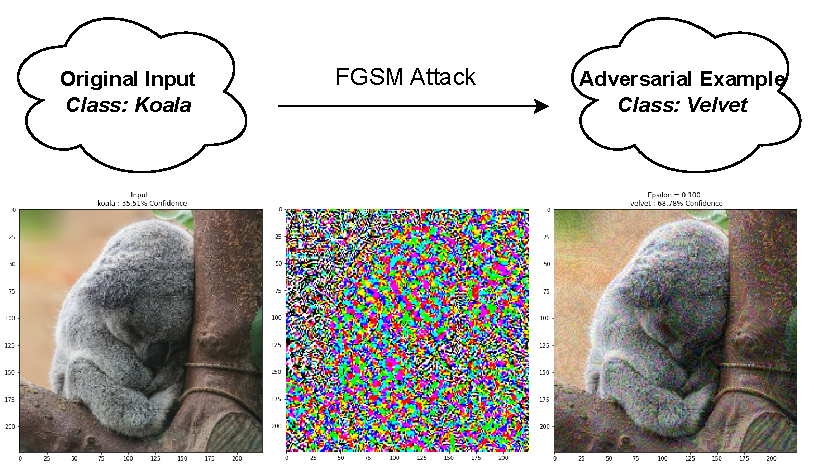
\includegraphics[width=\textwidth]{fig-koala_examples.pdf}
    \end{minipage}
    \begin{minipage}[b]{0.49\textwidth}
    \centering
    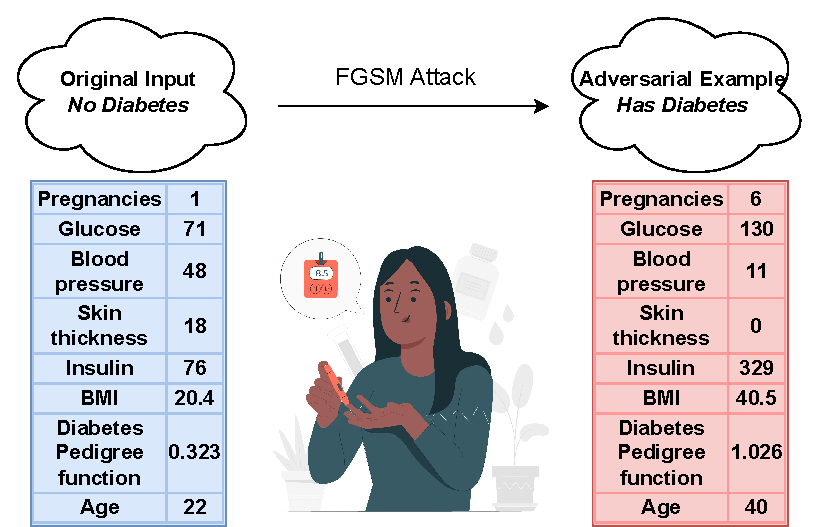
\includegraphics[width=\textwidth]{fig-diabetes_examples.pdf}
    \end{minipage}
    \end{center}
    
    \vspace{-0.8em}
    \textbf{\color{blue}Goal:} Develop a set of standardised properties and metrics to evaluate the imperceptibility of adversarial attacks on tabular data.

    % \vspace{0.3em}
    % \textbf{\color{blue}Key Contributions:}
    % \begin{itemize}
    %     \item Proposed a set of key properties and corresponding metrics designed to comprehensively characterise imperceptible adversarial attacks on tabular data. 
    %     \item Results indicate a trade-off between imperceptibility and attack effectiveness.
    %     \item Provides insights for improving adversarial algorithms.
    % \end{itemize}  
}

\headerbox{\bf\color{blue} Contributions and Findings}{name=finding,column=3,span=2}{
\textbf{\color{blue}Contributions:} Our contributions to the field are twofold:
\begin{itemize}
    \item We propose seven key properties that define imperceptible adversarial attacks for tabular data. These properties---\textit{\textbf{proximity}}, \textit{\textbf{sparsity}}, \textit{\textbf{deviation}}, \textit{\textbf{sensitivity}}, \textit{\textbf{immutability}}, \textit{\textbf{feasibility}}, and \textit{\textbf{feature interdependency}}---are derived from the unique characteristics and challenges associated with tabular data.
    \item Using the proposed metrics, we empirically evaluated five adversarial attack methods, investigating all seven imperceptibility properties, analysing their relationship with attack effectiveness, and providing insights from the results.

\end{itemize}

    \vspace{0.3em}
    \textbf{\color{blue}Findings:} The findings reveal that:

    \begin{itemize}
    \item With the exception of proximity, current adversarial attack methods often fail to consider the proposed imperceptibility properties in their algorithm designs.
    \item Additionally, our analysis highlights a trade-off between the effectiveness of adversarial attacks and their imperceptibility.
    \end{itemize}


%     \textbf{\color{blue}Adversarial Attack:} Consider a dataset where each input data point---a vector \(\bm{x} \in \mathbbm{X}\) belongs to a class with label \( y \in \mathbbm{Y}\). Let \(f(\cdot)\) denote a machine learning classifier, an adversarial example \(\bm{x}^{adv}\) generated by an adversarial attack is a perturbed input similar to \(\bm{x}\) and misclassifies the label of \(\bm{x}\).
%     \vspace{-0.5em}
%     \begin{equation*}
%     \bm{x}^{adv} = \bm{x} + \bm{\delta} \hspace{0.8em}\text{subject to }  f(\bm{x}^{adv})\neq y
%     \end{equation*} 
%     where \(\bm{\delta}\) denotes input perturbation.

%     \vspace{0.3em}
%     \textbf{\color{blue}Criteria for Imperceptibility:} 
%     Based on the nature of tabular data, we establish the following criteria in addressing imperceptibility of adversarial attacks on tabular data.
% \begin{itemize}
%     \item Minimisation of feature perturbation
%     \item Preservation of statistical data distribution
%     \item Narrow-guard feature perturbation
%     \item Preservation of feature semantics
%     \item Preservation of feature interdependencies
% \end{itemize}
}

%%%%%%%%%%%%%%%%%%%%%%%%%%%%%%%%%%%%%%%%%%%%%%%%%%%%%%%%%%%%%%%%%%%%%%%%%%%%%%%
\headerbox{\bf\color{blue} Properties and Metrics of Imperceptibility}{name=method,column=0,below=contribution,span=3}{

    % \begin{center}
    %     {\large \textit{\textbf{Quantitative Properties}}}
    % \end{center}

    \textbf{\color{blue}Proximity:} A good adversarial example should introduce \emph{minimal} changes, quantified by ensuring the smallest possible distance from the original feature vector. To measure the perturbation distance, we use the $\bm{\ell_2}$ and $\bm{\ell_\infty}$ \textbf{\textit{norms}}.
    % \begin{equation*}
    % \ell_p(\bm{x}^{adv},\bm{x})=\begin{cases}
    %       \Bigl(\sum_{i=1}^n(x^{adv}_i-x_i)^p \Bigr)^{1/p}, & p\in\{1,2\}\\
    %       \sup_{n}{\vert x^{adv}_n- x_n\vert}, & p \rightarrow \infty
    % \end{cases}
    % \end{equation*}

    \vspace{0.3em}
    \textbf{\color{blue}Sparsity:} An ideal adversarial example should misclassify the model's prediction by altering the fewest features possible. We use the $\bm{\ell_0}$ \textbf{\textit{norm}} to count the number of perturbed features.
    % \begin{equation*}
    %     Spa(\bm{x}^{adv}, \bm{x})=\sum_{i=1}^{n}\mathbbm{1}( x^{adv}_i-x_i)
    % \end{equation*}

    \vspace{0.3em}
    \textbf{\color{blue}Deviation:} To ensure imperceptibility, an adversarial example should closely resemble the majority of original inputs. We propose using the \textbf{\textit{Mahalanobis distance}} to measure the deviation between an adversarial perturbation and the distribution of variations in the original data inputs.
    % \begin{equation*}
    % \text{MD}(\bm{x}^{adv}, \bm{x})= \sqrt{(\bm{x}^{adv}-\bm{x})V^{-1}(\bm{x}^{adv}-\bm{x})^T}
    % \end{equation*}

    \vspace{0.3em}
    \textbf{\color{blue}Sensitivity:} We adapt the concept of \textit{\textbf{perturbation sensitivity}} as a metric to quantify the extent to which features with narrow distributions in tabular data are altered, which is defined as follows:
\vspace{-0.3em}
\begin{equation*}
       \text{SDV}(x_{i})= \sqrt{ \frac{ \sum^m_j ( x_{i,j}- \bar{x}_{i})^2 }{ m } }, \quad\text{SEN}(\bm{x}, \bm{x}^{adv})=\sum_{i=1}^n \frac{\Vert x^{adv}_{i} - x_{i} \Vert_2}{\text{SDV}(x_i)}
\vspace{-0.3em}
\end{equation*}
where $n$ is the number of numerical features, $m$ is the number of all input vectors, and $\bar{x}_{i}$ represents the average of the $i\text{th}$ features within all datapoints.
    

% \begin{center}
%     {\large \textit{\textbf{Qualitative Properties}}}
% \end{center}

\vspace{0.3em}
\textbf{\color{blue}Immutability:} \textbf{\textit{Immutable features}} are fixed attributes in a dataset that are either inherently unchangeable or should remain unaltered due to ethical or practical constraints.

\vspace{0.3em}
\textbf{\color{blue}Feasibility:} Adversarial attacks should avoid introducing perturbations that push feature values beyond \textbf{\textit{feasible value ranges}}, ensuring alignment with semantic correctness.

\vspace{0.3em}
\textbf{\color{blue}Feature Interdependency:} Tabular data often contains features with non-linear and context-specific interactions or relationships. Altering a feature independently of its \textbf{\textit{correlated features}} can create anomalies that are easily detectable.



}

%%%%%%%%%%%%%%%%%%%%%%%%%%%%%%%%%%%%%%%%%%%%%%%%%%%%%%%%%%%%%%%%%%%%%%%%%%%%%%
\headerbox{\bf\color{blue} Experiments \& Results}{name=results,column=3,below=contribution,span=2}{
    %\begin{minipage}[t]{0.5\textwidth}
        %\textbf{\color{blue}Synthetic Datasets for Training:} 
        %\vspace{-0.2em}
        %\begin{center}
        %    \includegraphics[width=\textwidth]{images/datasets.pdf}
        %\end{center}
    %\end{minipage}

        \textbf{\color{blue}Results of Attack Effectiveness:}
        \begin{center}
            \vspace{-0.8em}
            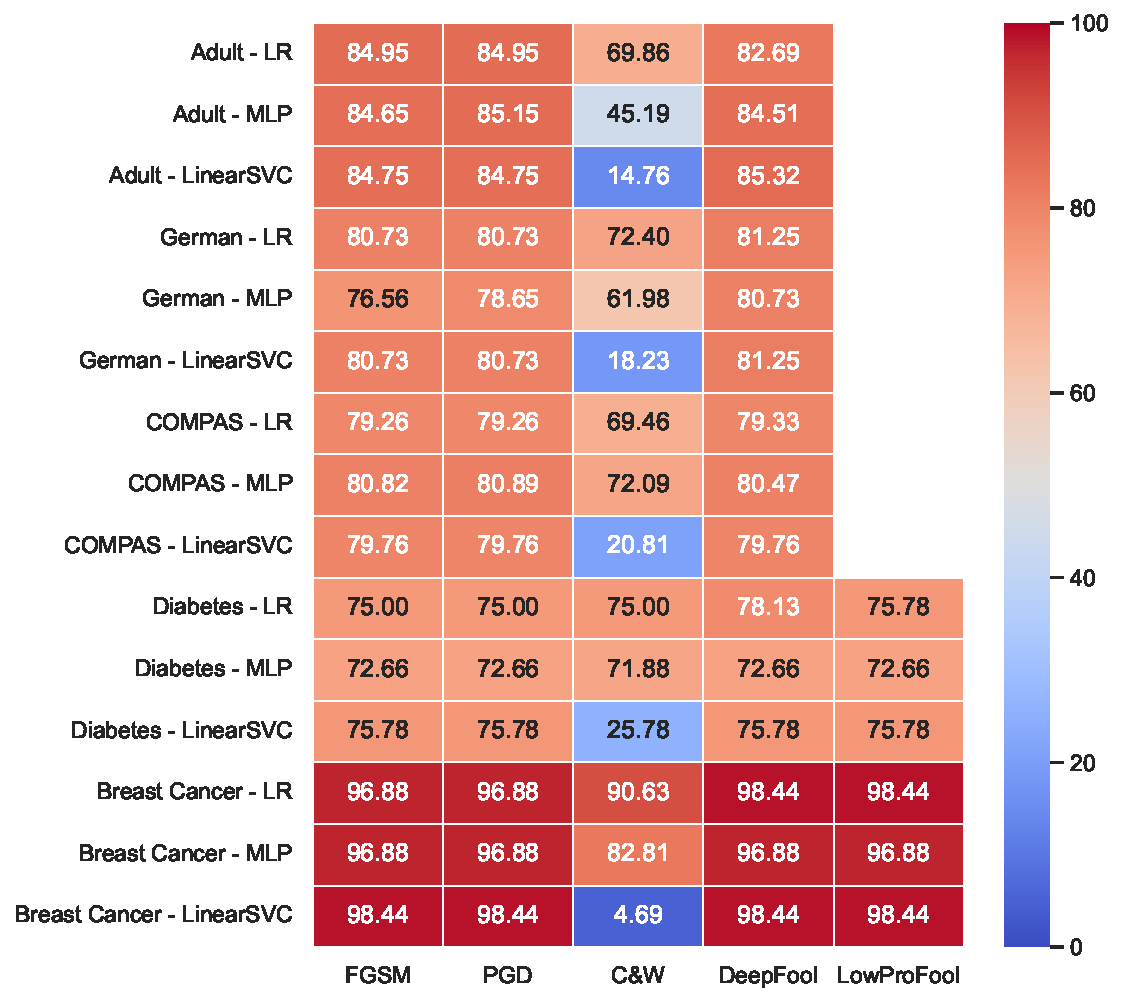
\includegraphics[width=\textwidth]{images/asr_rgb.pdf}
        \end{center}
        \vspace{-0.4em}
        \textbf{\color{blue}Results of Proxmity $\ell_2$:}
        \begin{center}
            \vspace{-0.7em}
            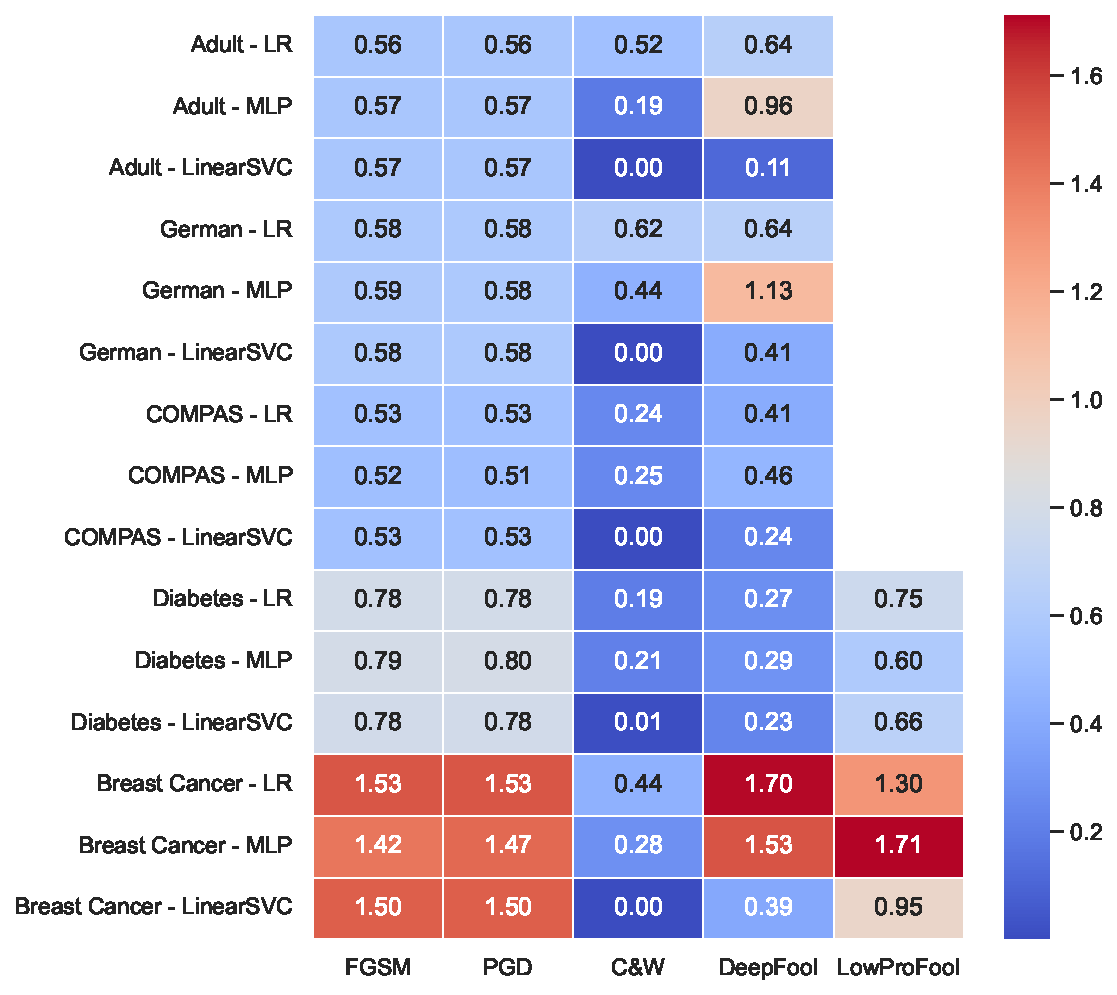
\includegraphics[width=\textwidth]{images/l2_rgb.pdf}
        \end{center}

    % \begin{minipage}[t]{0.48\textwidth}
    % \textbf{\color{blue}Results of Proximity $\ell_2$:}
    %     \begin{center}
    %         \vspace{-0.5em}
    %         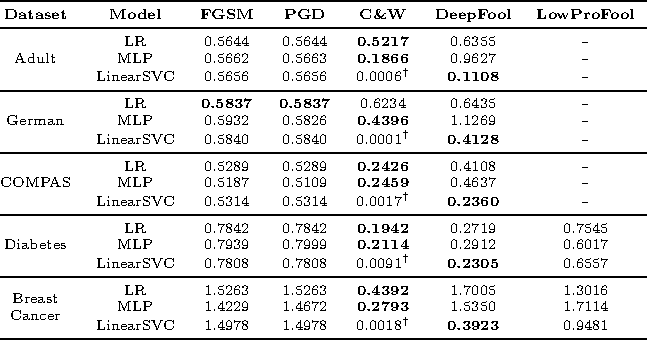
\includegraphics[width=\textwidth]{tables/tab-imperceptible_l2.pdf}
    %     \end{center}  
    
    % \end{minipage}


}

\headerbox{\bf\color{blue} Analysis of Imperceptibility using Qualitative Properties}{name=analysis,column=0,below=method,span=3}{

    \textbf{\color{blue}Immutability:} Feature \textit{Race} should not be perturbed. 

    \vspace{0.3em}
    \textbf{\color{blue}Feature Interdependency:}
    If feature \textit{Age}'s value is altered, feature \textit{Age Category} should be correspondingly updated to reflect this change accurately.
        \begin{center}
            \vspace{-0.3 em}
            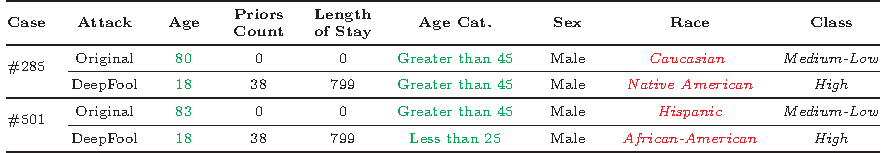
\includegraphics[width=0.98\textwidth]{tables/tab-immutable.pdf}
        \end{center} 

    \vspace{-0.5em}
        \textbf{\color{blue}Fessibility:} Features \textit{Glucose} and \textit{BMI} are prone to being perturbed into extreme values.
        \begin{center}
            \vspace{-0.3em}
            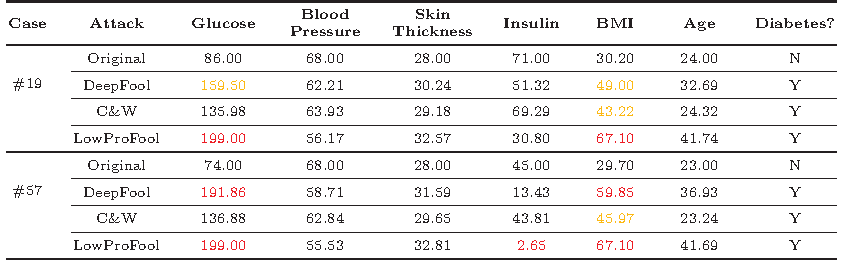
\includegraphics[width=0.98\textwidth]{tables/tab-feasibility.pdf}
        \end{center} 
}

%%%%%%%%%%%%%%%%%%%%%%%%%%%%%%%%%%%%%%%%%%%%%%%%%%%%%%%%%%%%%%%%%%%%%%%%%%%%%%
\headerbox{\bf\color{blue} About Us}{name=acknowledgment,column=3,below=results,span=2}{

        \begin{center}
        \begin{minipage}{0.56\linewidth}
            \begin{center}
            \textbf{Project Webpage}: \\
            \vspace{0.5em}\textbf{Code} \& \textbf{Dataset} \& \textbf{Model}
            \end{center}
        \end{minipage}
        \begin{minipage}{0.19\linewidth}
            \begin{center}
                
\includegraphics[width=\linewidth]{images/qr-code-github.png}
            \end{center}
        \end{minipage}
        \end{center}
}




\end{poster}
\end{document}
